%File: anonymous-submission-latex-2023.tex
\documentclass[letterpaper]{article} % DO NOT CHANGE THIS
\usepackage[submission]{aaai23}  % DO NOT CHANGE THIS
\usepackage{times}  % DO NOT CHANGE THIS
\usepackage{helvet}  % DO NOT CHANGE THIS
\usepackage{courier}  % DO NOT CHANGE THIS
\usepackage[hyphens]{url}  % DO NOT CHANGE THIS
\usepackage{graphicx} % DO NOT CHANGE THIS
\urlstyle{rm} % DO NOT CHANGE THIS
\def\UrlFont{\rm}  % DO NOT CHANGE THIS
\usepackage{natbib}  % DO NOT CHANGE THIS AND DO NOT ADD ANY OPTIONS TO IT
\usepackage{caption} % DO NOT CHANGE THIS AND DO NOT ADD ANY OPTIONS TO IT
\usepackage{subcaption} % DO NOT CHANGE THIS AND DO NOT ADD ANY OPTIONS TO IT
\frenchspacing  % DO NOT CHANGE THIS
\setlength{\pdfpagewidth}{8.5in} % DO NOT CHANGE THIS
\setlength{\pdfpageheight}{11in} % DO NOT CHANGE THIS
%
% These are recommended to typeset algorithms but not required. See the subsubsection on algorithms. Remove them if you don't have algorithms in your paper.
\usepackage[ruled,vlined,linesnumbered]{algorithm2e}

\usepackage{xcolor}

\setcounter{secnumdepth}{2} %May be changed to 1 or 2 if section numbers are desired.

\usepackage{xspace}
\newcommand{\plan}[1]{{\textcolor{blue}{[Plan: #1]}}}
\newcommand{\blocked}{\textit{blocked}}
\newcommand{\unblocked}{\textit{unblocked}}
\newcommand{\unknown}{\textit{b}|\textit{u}}
\newcommand{\assumeObs}{\textbf{AssumeObs}}
\newcommand{\toplan}{\textit{tree2plan}}
\newcommand{\po}{PO\xspace}
\newcommand{\pos}{POs\xspace}
\newcommand{\cons}{\textit{cons}}



% \newcommand{\tobranch}{\textit{plan2branch}}

\newcommand{\tuple}[1]{\ensuremath{\left \langle #1 \right \rangle }}

\newcommand{\guy}[1]{{\textcolor{red}{[Guy: #1]}}}
\newcommand{\Bar}[1]{{\textcolor{orange}{[Bar: #1]}}}
\newcommand{\roni}[1]{{\textcolor{green}{[Roni: #1]}}}

\newcommand{\commentout}[1]{}

\usepackage{amsthm,amsmath}

%\theoremstyle{definition}
\newtheorem{exmp}{Example}
\newtheorem{theorem}{Theorem}
\newtheorem{observation}{Observation}
\newtheorem{corollary}{Corollary}
\newtheorem{lemma}{Lemma}
\newtheorem{definition}{Definition}



%
% These are are recommended to typeset listings but not required. See the subsubsection on listing. Remove this block if you don't have listings in your paper.
\usepackage{newfloat}
\usepackage{listings}
\DeclareCaptionStyle{ruled}{labelfont=normalfont,labelsep=colon,strut=off} % DO NOT CHANGE THIS
\lstset{%
	basicstyle={\footnotesize\ttfamily},% footnotesize acceptable for monospace
	numbers=left,numberstyle=\footnotesize,xleftmargin=2em,% show line numbers, remove this entire line if you don't want the numbers.
	aboveskip=0pt,belowskip=0pt,%
	showstringspaces=false,tabsize=2,breaklines=true}
%\floatstyle{ruled}
%\newfloat{listing}{tb}{lst}{}
%\floatname{listing}{Listing}
%
% Keep the \pdfinfo as shown here. There's no need
% for you to add the /Title and /Author tags.
\pdfinfo{
/TemplateVersion (2023.1)
}

\title{Multi Agent Path Finding Under Obstacle Uncertainty --- Appendices}
\author{
    %Authors
    % All authors must be in the same font size and format.
    Written by AAAI Press Staff\textsuperscript{\rm 1}\thanks{With help from the AAAI Publications Committee.}\\
    AAAI Style Contributions by Pater Patel Schneider,
    Sunil Issar,\\
    J. Scott Penberthy,
    George Ferguson,
    Hans Guesgen,
    Francisco Cruz\equalcontrib,
    Marc Pujol-Gonzalez\equalcontrib
}
\affiliations{
    %Afiliations
    \textsuperscript{\rm 1}Association for the Advancement of Artificial Intelligence\\
    % If you have multiple authors and multiple affiliations
    % use superscripts in text and roman font to identify them.
    % For example,

    % Sunil Issar, \textsuperscript{\rm 2}
    % J. Scott Penberthy, \textsuperscript{\rm 3}
    % George Ferguson,\textsuperscript{\rm 4}
    % Hans Guesgen, \textsuperscript{\rm 5}.
    % Note that the comma should be placed BEFORE the superscript for optimum readability

    1900 Embarcadero Road, Suite 101\\
    Palo Alto, California 94303-3310 USA\\
    % email address must be in roman text type, not monospace or sans serif
    publications23@aaai.org
%
% See more examples next
}

%Example, Single Author, ->> remove \iffalse,\fi and place them surrounding AAAI title to use it
\iffalse
\title{My Publication Title --- Single Author}
\author {
    Author Name
}
\affiliations{
    Affiliation\\
    Affiliation Line 2\\
    name@example.com
}
\fi

\iffalse
%Example, Multiple Authors, ->> remove \iffalse,\fi and place them surrounding AAAI title to use it
\title{My Publication Title --- Multiple Authors}
\author {
    % Authors
    First Author Name,\textsuperscript{\rm 1}
    Second Author Name, \textsuperscript{\rm 2}
    Third Author Name \textsuperscript{\rm 1}
}
\affiliations {
    % Affiliations
    \textsuperscript{\rm 1} Affiliation 1\\
    \textsuperscript{\rm 2} Affiliation 2\\
    firstAuthor@affiliation1.com, secondAuthor@affilation2.com, thirdAuthor@affiliation1.com
}
\fi


% REMOVE THIS: bibentry
% This is only needed to show inline citations in the guidelines document. You should not need it and can safely delete it.
\usepackage{bibentry}
% END REMOVE bibentry

\begin{document}

\maketitle



\section{Theorems with Proofs}

\begin{definition}[MAPFOU Constraint]
A MAPFOU constraint is defined by a tuple $\tuple{i,v,t,c_i,c_j}$ 
where $i$ is an agent, 
$v$ is a vertex,
$t$ is a time step, 
and $c_i$ and $c_j$ are obstacle configurations. 
A plan tree $\tau$ satisfies a MAPFOU constraint if one of the following conditions holds:
\begin{eqnarray}
(C1) ~~~ \forall p\in O&:& \left(c(p)=c_i(p)\right)\vee \left(c(p)=\unknown\right) \\
(C2) ~~~ \forall p\in O&:& c_i(p)\neq\unknown \rightarrow c(p)=c_i(p) ~ \wedge  \\
 &&   c_i(p)=\unknown \rightarrow c(p)=c_j(p)
\end{eqnarray}
\label{def:mapfou-constraint}
\end{definition}

\begin{observation}
For any MAPFTOU problem $\mathcal{P}$, if $\{\tau_i\}$ is an optimal solution wrt 
the best-case SOC objective function then its cost is equal to the SOC of the single-agent plans corresponding to the obstacle configuration where all potential obstacles are \unblocked. 
Similarly, the optimal worst-case SOC is equal to the SOC of the single-agent plans corresponding to the obstacle configuration where all potential obstacles are \blocked. 
\label{obs:best-and-worst}
\end{observation}

\begin{observation}
Plan trees $\tau^i$ and $\tau^j$ have a conflict 
iff there exists two nodes $n^i\in\tau^i$ and $n^j\in\tau^j$ that form conflict. 
\label{obs:conditionsForConflicts}
\end{observation} 

\begin{theorem}
Given a sound, complete, and optimal CMAPF solver, CEBC and CEWC algorithms are also sound, complete, and optimal, i.e., guaranteed to return a solution, if such exists, which has no conflicts and is optimal wrt to the chosen objective function (best- or worst-case SOC).
\end{theorem}


\begin{proof}
\noindent \textbf{Soundness.}
Every branch in the plan trees returned by our algorithm is created by running a CMAPF solver under the assumption of a specific obstacle configuration for all agents. 
As the CMAPF solver is sound, the branches of the plan trees do not contain any conflict, and all agents end at the goal in that branch. In addition, the main loop (lines 6-15) ends after inspecting all actions in the active branch, and hence the plan tree does not contain any unexplored branches. 
Thus, the solution is sound, i.e., conflict-free and in all leaves, all agents reached their target.

\noindent\textbf{Completeness.} 
As the underlying graph $G$ is undirected and sensing actions do not change it, the agents can always backtrack to any joint state they occupied before. Thus, adding nodes and edges to the plan trees never results in a dead-end. 
The number of potential obstacles in finite and every recursive call to our algorithm removes one potential conflict from $U$. Hence, we are a guaranteed that our algorithm terminates in finite time. 

\noindent\textbf{Optimality.} Consider the the best-case SOC objective function. We know that the optimal best-case SOC is equal to the solution of the CMAPF problem that corresponds to assuming all potential obstacles are unblocked (Observation~\ref{obs:best-and-worst}). By construction, our algorithm is guaranteed to include that solution as branches in the resulting set of plan trees. 
\end{proof}



\begin{theorem}
DEBC is sound, complete, and optimal. 
\label{the:debc-optimal}
\end{theorem}

\begin{proof}
Soundness is trivially guaranteed because only solutions without conflicts are returned. 
To prove completeness and optimality in the same way given for the standard CBS-based algorithms~\cite{sharon2015conflict,atzmon2020robust,li2020new}, we must prove that the pair of constraints we impost when a conflict is detected is \emph{sound}~\cite{atzmon2020robust,li2020new}. 
That is, the constraints we impose do not preclude reaching any (conflict-free) solution. 
To see this, consider a conflict formed by a pair of plan tree nodes
$n^i$ and $n^j$ at vertex $v$ and time $t$ with obstacle configurations $c_i$ and $c_j$, respectively. 
The corresponding MAPFOU constraints are $\tuple{i,v,t,c_i,c_j}$
and $\tuple{j,v,t,c_j,c_j}$. 
We will now show that any solution to the given MAPFOU solution must satisfy at least one of these constraints. 
We prove this by negation: let $\{\hat{\tau}^i\}_i$ be a (conflict-free) solution that does not satisfy both constraints. 
This means the plan trees $\hat{\tau}^i$ and $\hat{\tau}^j$
include nodes 
$\hat{n}^j$ and
$\hat{n}^i$, respectively, 
where $\hat{n}^i.v=v$, $\hat{n}^i.t=t$, 
and $\hat{n}^i.c$ and $\hat{n}^j.c$
satisfy either (C1) or (C2) from Definition~\ref{def:mapfou-constraint}
for their respective constraints. 
Thus, either both nodes satisfy (C1), both satisfy (C2), or one satisfies (C1) and the other (C2).  
For each of these cases, $\hat{n}^i.c$ and $\hat{n}^j.c$ ends up being consistent, which means that $\hat{n}^i$ and $\hat{n}^j$ form a conflict, contradicting the assumption that $\{\hat{\tau}^i\}_i$ is a (conflict-free) solution. 
\end{proof}

% RONI: COMMENTED OUT A NICE VERSION OF THE PROOF
% Let $C1(C)$ and $C2(C)$ be all the obstacle configurations that satisfy condition C1 and C2, respectively, wrt the MAPOU constrain $C$.
% That is, 
% \begin{scriptsize}
% \begin{eqnarray*}
% \scriptsize
% C1(\tuple{i,v,t,c_i,c_j}) =  \{c|\forall p\in O: \left(c(p)=c_i(p)\right)\vee \left(c(p)=\unknown\right)\}\\
% C2(\tuple{i,v,t,c_i,c_j}) = \{c|\forall p\in O: c_i(p)\neq\unknown \rightarrow c(p)=c_i(p) \\
%  ~~~~~ \wedge c_i(p)=\unknown \rightarrow c(p)=c_j(p)\} 
% \end{eqnarray*}
% \end{scriptsize}
% For a conflict formed by nodes $n^i$ and $n^j$, let $C^i$ and $C^j$ be the respective constraints, i.e., 
% $C^i=\tuple{i,v,t,c_i,c_j})$ and $C^j=\tuple{j,v,t,c_j,c_i})$. 
% A plan tree for agent $i$ satisfies constraint $C^i$ if every node $n$ for which $n.v=v$ and $n.t=t$ must not have an obstacle configuration in $c\in C1(C^i)\cup C2(C^i)$. 
% The key to the proof is the following observation:
% \begin{observation}
% For any pair of obstacle configurations $c_i$ and $c_j$ that are consistent, 
% it holds that every pair of obstacle configuration 
% $c^i\in  C1(C^i)\cup C2(C^i)$ and 
% $c^j\in  C1(C^j)\cup C2(C^j)$ 
% are also consistent. 
% \label{obs:consistency-relation}
% \end{observation}
% \roni{I can prove this observation if needed}
% Now, consider a solution that does not satisfy $C^i$ and $C^j$. 
% This means there exists a pair of nodes $\hat{n}^i$ and $\hat{n}^j$ in the respective plan trees of agents $i$ and $j$, where (1) $\hat{n}^i.v=\hat{n}^j.v=v$, 
% (2) $\hat{n}^i.t=\hat{n}^j.t=t$, 
% (3) $\hat{n}^i.c\in C1(C^i)\cup C2(C^i)$, 
% and (4) $\hat{n}^j.c\in C1(C^j)\cup C2(C^j)$.
% Due to Observation~\ref{obs:consistency-relation}, we know that 
% $\hat{n}^i.c$ 
% and 
% $\hat{n}^j.c$
% are consistent, 
% and thus $\hat{n}^i$ and $\hat{n}^j$ form a conflict. 


\section{Appendix 2 - Centralized Execution Worst Case Algorithm}

\begin{algorithm}[t]
\caption{Centralized Execution, Worst Case (CEWC)}
    \label{alg:CEWC}
\footnotesize
\SetKwBlock{CEWC}{CEWC}{end}
\SetKwInOut{Input}{Input: }
\SetKwInOut{Output}{Output: }
\CEWC{
\Input{Grid $G$, Known obstacles $K$, Unknown obstacles $U$, Start positions $S$, Target positions $T$}
    $G' \leftarrow $ A grid identical to $G$ where all vertices in $U$ are blocked, and all vertices in $K$ are as observed\\
    $\Pi \leftarrow PlanCMAPF(G',S,T)$\\

    For every agent $i$, create a sequence of nodes $n^i_j$ corresponding to the vertices in $\pi^i$, marking all edges using the null observation\\
    $K' \leftarrow \emptyset$\\
    \For{$j=1...\max(|\pi^i|)-1$}{
        Find $p$ s.t. $p \in U \setminus K', \exists i : \langle p, n^i_{j}.p \rangle \in E$\\
        \If{there exists such $p$}{
            $\{\tau^k \} \leftarrow CEWC(G,K \cup \{blocked(p'):p' \in K'\} \cup \{unblocked(p)\},U \setminus (K' \cup \{p\}), \{n^l_j.p : \textrm{for every agent } l\}, T)$ \\
            \For{every agent $k$}{
                Add a new node $n_{sense}$ with action $Sense(p)$ before $n^k_j$\\
                Add an outgoing edge from $n_{sense}$, marked $blocked(p)$, with child $n^k_j$\\
                Add an outgoing edge from $n_{sense}$, marked $unblocked(p)$, with child $\tau^k$\\
            }
            Add $p$ to $K'$\\
        }
    }
    For every agent $i$, create plan tree $\tau^i$, with root $n^i_1$\\
    \Return{$\{ \tau^i \}$}
}
\end{algorithm}

Algorithm~\ref{alg:CEWC}, optimizing for the worst case, i.e., when all obstacles are assumed to be blocked, is very similar. CEWC (centralized execution worst case) differs from CEBC (Algorithm~\ref{alg:CEBC}) in that we assume, in the CMAPF problem (line 2) that all unobserved vertices are blocked. The recursive call (line 9), assumes that $p$ is unblocked, allowing a possible shortcut over the worst case. The children of the sensing nodes are also attached to the opposite case than in CEBC. 

\section{Decentralized Execution - Algorithm and Example}


 \begin{algorithm}[t]
 \caption{Single agent best case (SABC)}
     \label{alg:SABC}
 \footnotesize
 \SetKwBlock{SABC}{SABC}{end}
 \SetKwBlock{Main}{Main}{end}
 \SetKwInOut{Input}{Input: }
 \SetKwInOut{Output}{Output: }
 \SABC{
 \Input{Graph $G$, start vertex $S^i$, target vertex $T^i$}
 \Input{Partial obstacle configuration $K$}
 \Input{Unknown potential obstacles $U$}
 \Input{Agent $i$, Constraint $C$}
     $G' \gets \assumeObs(G, K\cup\{v:\unblocked|v\in U\})$\\
     $\pi^i \leftarrow A^*(G',S_i,T_i,C)$\\
     $(n^i_1,\ldots,n_{|\pi^i|}^i)\gets \textbf{CreateBranch}(\pi^i)$\\
     \For{$j=1...\max(|\pi^i|)-1$}{
         Find $p\in U$ s.t. $p\notin K\wedge \exists i: \tuple{p,n^i_j.p}\in E$\\
         \If{there exists such $p$}{
             $\tau' \leftarrow SABC(G, n^i_j.p, T_i,  
             K \cup \{p:\blocked\}, U \setminus \{p\}, 
             i, C)$\\
             Add a new node $n_{sense}$ with action $Sense(p)$ before $n^i_j$\\
             Add an outgoing edge from $n_{sense}$, marked $unblocked(p)$, with child $n^i_j$\\
             Add an outgoing edge from $n_{sense}$, marked $blocked(p)$, with child $\tau'$\\
             Add $p:\blocked$ to $K$\\
             Remove $p$ from $U$
         }
     }
     Create plan tree $\tau^i$, with root $n^i_1$\\
     \Return $\tau^i$
 }
 \Main{
     SABC$(G,s_i, t_i, \emptyset, O, i, C)$
 }
 \end{algorithm}




Algorithm~\ref{alg:SABC} shows the pseudo-code for building a plan tree for a single agent aiming to optimizie the best-case SOC. 
 It is similar to our CEBC algorithm, except that we use a single-agent solver ($A^*$) instead of a CMAPF solver to generate single-agent plans, and it can accept constraints of the form $\langle v, t \rangle$, forbidding the agent to be at vertex $v$ at time $t$. These constraints are passed directly to the single-agent solver, which ensures that they are satisfied. 


We begin by creating a CMAPF problem as in the CEBC algorithms (line 2). 
We use here single agent $A^*$ instead of CBS (line 3). $A^*$ receives as input a set of constraints of the form $\langle v, t \rangle$, forbidding the agent to be at vertex $v$ at time $t$. 
Similar to the algorithms above, we traverse the resulting branch, calling recursively to SABC for blocked observations (line 9).

Worst-case (SAWC) is similar, assuming that all unobserved vertices are blocked (line 2), and modifying the recursive call (line 9), and the child nodes linking (lines 11-12), as in CEWC.




\begin{figure}[t]
    \begin{subfigure}[b]{0.4\textwidth}
      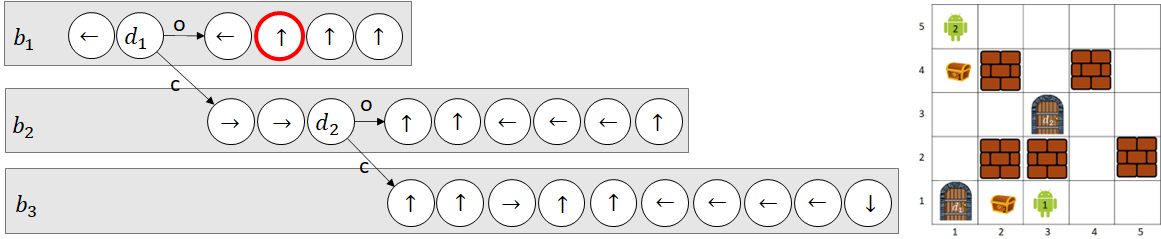
\includegraphics[scale=.25]{Figures/DEBC1.1+example.png}
      \caption{DEBC, Agent 1, Iteration 1}
      \label{fig:DEBC1.1}
    \end{subfigure}
    \begin{subfigure}[b]{0.4\textwidth}
      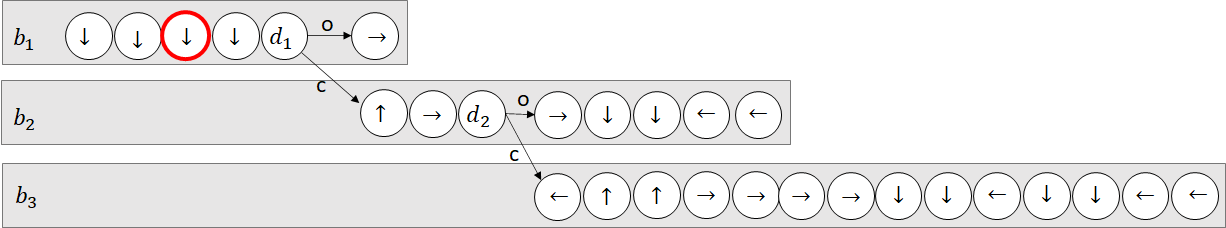
\includegraphics[scale=.25]{Figures/DEBC2.1.png}
      \caption{DEBC, Agent 2, Iteration 1}
      \label{fig:DEBC2.1}
    \end{subfigure}
    \hrule\vspace{5pt}\par
    \begin{subfigure}[b]{0.4\textwidth}
      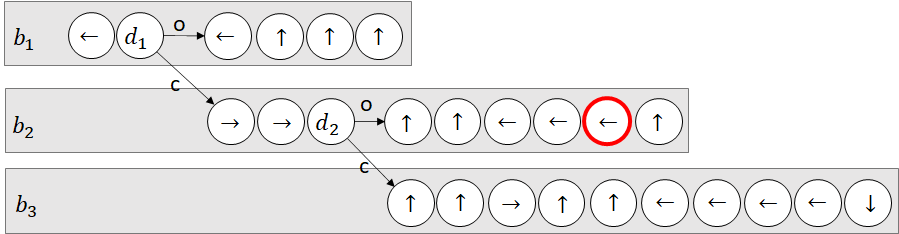
\includegraphics[scale=.25]{Figures/DEBC1.2.png}
      \caption{DEBC, Agent 1, Iteration 2}
      \label{fig:DEBC1.2}
    \end{subfigure}
    \begin{subfigure}[b]{0.4\textwidth}
      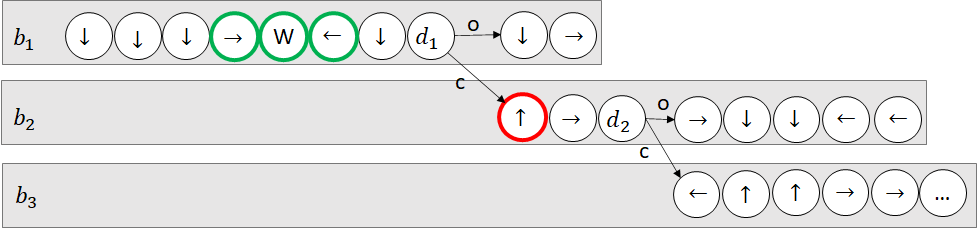
\includegraphics[scale=.25]{Figures/DEBC2.2.png}
      \caption{DEBC, Agent 2, Iteration 2}
      \label{fig:DEBC2.2}
    \end{subfigure}   
    \hrule\vspace{5pt}\par
    \begin{subfigure}[b]{0.4\textwidth}
      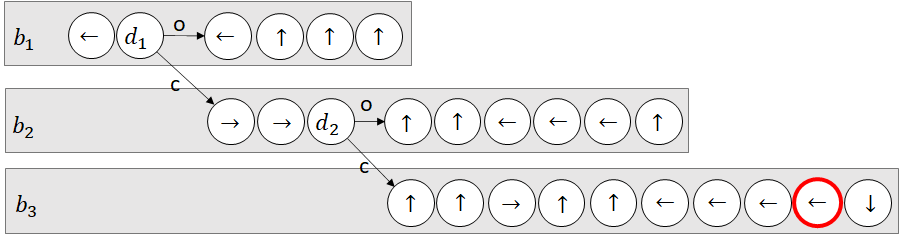
\includegraphics[scale=.25]{Figures/DEBC1.3.png}
      \caption{DEBC, Agent 1, Iteration 3}
      \label{fig:DEBC1.3}
    \end{subfigure}
    \begin{subfigure}[b]{0.4\textwidth}
      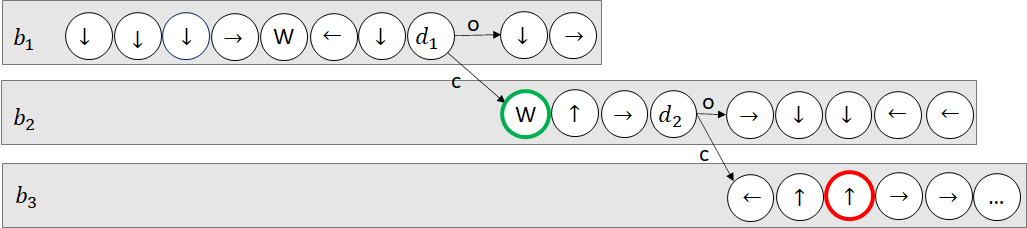
\includegraphics[scale=.25]{Figures/DEBC2.3.png}
      \caption{DEBC, Agent 2, Iteration 3}
      \label{fig:DEBC2.3}
    \end{subfigure}
    \caption{Plan trees for DEBC over the running example. Arrows denote movement actions, $W$ denotes waiting, $d_i$ denote sensing whether door $i$ is open or closed, $o,c$ denote the open and closed observations. Red nodes denote conflicts, and green nodes denote conflict resolutions.}
    \label{fig:DEBC}
\end{figure}


\begin{exmp}
Figure~\ref{fig:DEBC} demonstrates a part of the DEBC process for our running example. We focus here not on the creation of plan trees, but rather on conflict identification and resolution. After the first iteration of plan tree construction we get the trees in Figures~\ref{fig:DEBC1.1} and \ref{fig:DEBC2.1}. As we can see, each agent plans independently, and hence, the trees split at different times. We now look for possible conflicts, and identify that both agents at time $3$ arrive at vertex $\langle 1, 2 \rangle$ (above $d_1$). We now check the nodes for consistency. The node for agent 1 is after observing $open(d_1)$, while the node for agent 2 is before any observations. However, the observations sets $\{open(d_1)\}$ and $\emptyset$ are consistent, and hence, a collision may occur.

As the collisions occurred before any closed doors were observed, we must replan from scratch. We replan for agent 1 with the constraint $[ 1, \langle 1, 2 \rangle, 3 ] $, and for agent 2 with the constraint $[ 2, \langle 1, 2 \rangle, 3 ] $. 

We now proceed with CBS following the replanning of agent 2 (Figures~\ref{fig:DEBC1.2} and \ref{fig:DEBC2.2}). Green nodes represent the detour that agent 2 had to take to avoid the collision. We now observe another collision, at vertex $\langle 1,3 \rangle $. Now, the observations for agent 1 at the collision point are $\{closed(d_1),open(d_2)\}$ and the observations for agent 2 are $\{closed(d_1)\}$. Again, these sets are consistent, and we must resolve the conflict. We again create two constraints and replan.
Figures~\ref{fig:DEBC1.3} and \ref{fig:DEBC2.3} show the result after replanning for agent 2. Again, we added a wait to avoid the conflict, and a new collision is detected at a later branch, and needs to be resolved.

\end{exmp}



\bibliography{aaai23}


\end{document}